%  A simple AAU report template.
%  2015-05-08 v. 1.2.0
%  Copyright 2010-2015 by Jesper Kjær Nielsen <jkn@es.aau.dk>
%
%  This is free software: you can redistribute it and/or modify
%  it under the terms of the GNU General Public License as published by
%  the Free Software Foundation, either version 3 of the License, or
%  (at your option) any later version.
%
%  This is distributed in the hope that it will be useful,
%  but WITHOUT ANY WARRANTY; without even the implied warranty of
%  MERCHANTABILITY or FITNESS FOR A PARTICULAR PURPOSE.  See the
%  GNU General Public License for more details.
%
%  You can find the GNU General Public License at <http://www.gnu.org/licenses/>.
%
%  A simple AAU report template.
%  2015-05-08 v. 1.2.0
%  Copyright 2010-2015 by Jesper Kjær Nielsen <jkn@es.aau.dk>
%
%  This is free software: you can redistribute it and/or modify
%  it under the terms of the GNU General Public License as published by
%  the Free Software Foundation, either version 3 of the License, or
%  (at your option) any later version.
%
%  This is distributed in the hope that it will be useful,
%  but WITHOUT ANY WARRANTY; without even the implied warranty of
%  MERCHANTABILITY or FITNESS FOR A PARTICULAR PURPOSE.  See the
%  GNU General Public License for more details.
%
%  You can find the GNU General Public License at <http://www.gnu.org/licenses/>.
%
\documentclass[11pt,twoside,a4paper,openright]{report}
%%%%%%%%%%%%%%%%%%%%%%%%%%%%%%%%%%%%%%%%%%%%%%%%
% Language, Encoding and Fonts
% http://en.wikibooks.org/wiki/LaTeX/Internationalization
%%%%%%%%%%%%%%%%%%%%%%%%%%%%%%%%%%%%%%%%%%%%%%%%
% Select encoding of your inputs. Depends on
% your operating system and its default input
% encoding. Typically, you should use
%   Linux  : utf8 (most modern Linux distributions)
%            latin1 
%   Windows: ansinew
%            latin1 (works in most cases)
%   Mac    : applemac
% Notice that you can manually change the input
% encoding of your files by selecting "save as"
% an select the desired input encoding. 
\usepackage[utf8]{inputenc}
% Make latex understand and use the typographic
% rules of the language used in the document.
\usepackage[english]{babel}
% Use the palatino font
\usepackage[sc]{mathpazo}
\linespread{1.05}         % Palatino needs more leading (space between lines)
% Choose the font encoding
\usepackage[T1]{fontenc}
%%%%%%%%%%%%%%%%%%%%%%%%%%%%%%%%%%%%%%%%%%%%%%%%
% Graphics and Tables
% http://en.wikibooks.org/wiki/LaTeX/Importing_Graphics
% http://en.wikibooks.org/wiki/LaTeX/Tables
% http://en.wikibooks.org/wiki/LaTeX/Colors
%%%%%%%%%%%%%%%%%%%%%%%%%%%%%%%%%%%%%%%%%%%%%%%%
% load a colour package
\usepackage{xcolor}
\definecolor{aaublue}{RGB}{33,26,82}% dark blue
% The standard graphics inclusion package
\usepackage{graphicx}
% Set up how figure and table captions are displayed
\usepackage{caption}
\captionsetup{%
  font=footnotesize,% set font size to footnotesize
  labelfont=bf % bold label (e.g., Figure 3.2) font
}
% Make the standard latex tables look so much better
\usepackage{array,booktabs}
% Enable the use of frames around, e.g., theorems
% The framed package is used in the example environment
\usepackage{framed}
\usepackage{tikz}
\usetikzlibrary{shapes,shadows}
%%%%%%%%%%%%%%%%%%%%%%%%%%%%%%%%%%%%%%%%%%%%%%%%
% Mathematics
% http://en.wikibooks.org/wiki/LaTeX/Mathematics
%%%%%%%%%%%%%%%%%%%%%%%%%%%%%%%%%%%%%%%%%%%%%%%%
% Defines new environments such as equation,
% align and split 
\usepackage{amsmath}
% Adds new math symbols
\usepackage{amssymb}
% Use theorems in your document
% The ntheorem package is also used for the example environment
% When using thmmarks, amsmath must be an option as well. Otherwise \eqref doesn't work anymore.
\usepackage[framed,amsmath,thmmarks]{ntheorem}

%%%%%%%%%%%%%%%%%%%%%%%%%%%%%%%%%%%%%%%%%%%%%%%%
% Page Layout
% http://en.wikibooks.org/wiki/LaTeX/Page_Layout
%%%%%%%%%%%%%%%%%%%%%%%%%%%%%%%%%%%%%%%%%%%%%%%%
% Change margins, papersize, etc of the document
\usepackage[
  inner=28mm,% left margin on an odd page
  outer=41mm,% right margin on an odd page
  ]{geometry}
% Modify how \chapter, \section, etc. look
% The titlesec package is very configureable
\usepackage{titlesec}
\titleformat{\chapter}[hang]{\normalfont\huge\bfseries}{\chaptertitlename\ \thechapter}{20pt}{\Huge}
\titleformat*{\section}{\normalfont\Large\bfseries}
\titleformat*{\subsection}{\normalfont\large\bfseries}
\titleformat*{\subsubsection}{\normalfont\normalsize\bfseries}
%\titleformat*{\paragraph}{\normalfont\normalsize\bfseries}
%\titleformat*{\subparagraph}{\normalfont\normalsize\bfseries}

% Title spacing/margins {left}{top}{bottom}
\titlespacing{\chapter}{0pt}{-20pt}{10pt}  

% Clear empty pages between chapters
\let\origdoublepage\cleardoublepage
\newcommand{\clearemptydoublepage}{%
  \clearpage
  {\pagestyle{empty}\origdoublepage}%
}
\let\cleardoublepage\clearemptydoublepage

% Change the headers and footers
\usepackage{fancyhdr}
\pagestyle{fancy}
\fancyhf{} %delete everything
\renewcommand{\headrulewidth}{0pt} %remove the horizontal line in the header
\fancyhead[RE]{\small\nouppercase\leftmark} %even page - chapter title
\fancyhead[LO]{\small\nouppercase\rightmark} %uneven page - section title
\fancyfoot[C]{\thepage} %page number on all pages
% Do not stretch the content of a page. Instead,
% insert white space at the bottom of the page
\raggedbottom
% Enable arithmetics with length. Useful when
% typesetting the layout.
\usepackage{calc}

% Table of Contents depth: 0=chapter, 1=section...
\setcounter{tocdepth}{1}

%%%%%%%%%%%%%%%%%%%%%%%%%%%%%%%%%%%%%%%%%%%%%%%%
% Bibliography
% http://en.wikibooks.org/wiki/LaTeX/Bibliography_Management
%%%%%%%%%%%%%%%%%%%%%%%%%%%%%%%%%%%%%%%%%%%%%%%%
\usepackage[backend=bibtex,natbib=true,sorting=none]{biblatex} 
\addbibresource{Bibliography/MainBibliography.bib}

%%%%%%%%%%%%%%%%%%%%%%%%%%%%%%%%%%%%%%%%%%%%%%%%
% Misc
%%%%%%%%%%%%%%%%%%%%%%%%%%%%%%%%%%%%%%%%%%%%%%%%
% Add bibliography and index to the table of
% contents
\usepackage[nottoc]{tocbibind}
% Add the command \pageref{LastPage} which refers to the
% page number of the last page
\usepackage{lastpage}
% Add todo notes in the margin of the document
\usepackage[
%  disable, %turn off todonotes
  colorinlistoftodos, %enable a coloured square in the list of todos
  textwidth=\marginparwidth, %set the width of the todonotes
  textsize=scriptsize, %size of the text in the todonotes
  ]{todonotes}

\usepackage{parskip}

%%%%%%%%%%%%%%%%%%%%%%%%%%%%%%%%%%%%%%%%%%%%%%%%
% Hyperlinks
% http://en.wikibooks.org/wiki/LaTeX/Hyperlinks
%%%%%%%%%%%%%%%%%%%%%%%%%%%%%%%%%%%%%%%%%%%%%%%%
% Enable hyperlinks and insert info into the pdf
% file. Hypperref should be loaded as one of the 
% last packages
\usepackage{hyperref}
\hypersetup{%
	pdfpagelabels=true,%
	plainpages=false,%
	pdfauthor={Author(s)},%
	pdftitle={Title},%
	pdfsubject={Subject},%
	bookmarksnumbered=true,%
	colorlinks=false,%
	citecolor=black,%
	filecolor=black,%
	linkcolor=black,% you should probably change this to black before printing
	urlcolor=black,%
	pdfstartview=FitH%
}% package inclusion and set up of the document
% \gls{} acronyms
% \newacronym{tiae}{TIAE}{This Is An Example}
\newacronym{astep}{aSTEP}{AAU Spatio-Temporal data management Platform}
\newacronym{rs}{Ramsy}{Rideshare Automatic Matching System}
\newacronym{ui}{UI}{user interface}


%%%%%%%%%%%%%%%%%%%%%%%%%%%%%%%%%%%%%%%%%%%%%%%%%%%%%%%%%%%%%%%%%
% see, e.g., http://en.wikibooks.org/wiki/LaTeX/Formatting#Hyphenation
% for more information on word hyphenation
\hyphenation{ex-am-ple hy-phen-a-tion short}
\hyphenation{long la-tex}% 
%  A simple AAU report template.
%  2015-05-08 v. 1.2.0
%  Copyright 2010-2015 by Jesper Kjær Nielsen <jkn@es.aau.dk>
%
%  This is free software: you can redistribute it and/or modify
%  it under the terms of the GNU General Public License as published by
%  the Free Software Foundation, either version 3 of the License, or
%  (at your option) any later version.
%
%  This is distributed in the hope that it will be useful,
%  but WITHOUT ANY WARRANTY; without even the implied warranty of
%  MERCHANTABILITY or FITNESS FOR A PARTICULAR PURPOSE.  See the
%  GNU General Public License for more details.
%
%  You can find the GNU General Public License at <http://www.gnu.org/licenses/>.
%
%
%
% see, e.g., http://en.wikibooks.org/wiki/LaTeX/Customizing_LaTeX#New_commands
% for more information on how to create macros

%%%%%%%%%%%%%%%%%%%%%%%%%%%%%%%%%%%%%%%%%%%%%%%%
% Macros for the titlepage
%%%%%%%%%%%%%%%%%%%%%%%%%%%%%%%%%%%%%%%%%%%%%%%%
%Creates the aau titlepage
\newcommand{\aautitlepage}[3]{%
  {
    %set up various length
    \ifx\titlepageleftcolumnwidth\undefined
      \newlength{\titlepageleftcolumnwidth}
      \newlength{\titlepagerightcolumnwidth}
    \fi
    \setlength{\titlepageleftcolumnwidth}{0.5\textwidth-\tabcolsep}
    \setlength{\titlepagerightcolumnwidth}{\textwidth-2\tabcolsep-\titlepageleftcolumnwidth}
    %create title page
    \thispagestyle{empty}
    \noindent%
    \begin{tabular}{@{}ll@{}}
      \parbox{\titlepageleftcolumnwidth}{
        
\includegraphics[width=\titlepageleftcolumnwidth]{figures/aau_logo_en}
      } &
      \parbox{\titlepagerightcolumnwidth}{\raggedleft\sf\small
        #2
      }\bigskip\\
       #1 &
      \parbox[t]{\titlepagerightcolumnwidth}{%
      \textbf{Abstract:}\bigskip\par
        \fbox{\parbox{\titlepagerightcolumnwidth-2\fboxsep-2\fboxrule}{%
          #3
        }}
      }\\
    \end{tabular}
    \vfill
    \noindent{\footnotesize\emph{The content of this report is freely available, but publication (with reference) may only be pursued due to agreement with the author.}}
    \clearpage
  }
}

%Create english project info
\newcommand{\englishprojectinfo}[8]{%
  \parbox[t]{\titlepageleftcolumnwidth}{
    \textbf{Title:}\\ #1\bigskip\par
    \textbf{Theme:}\\ #2\bigskip\par
    \textbf{Project Period:}\\ #3\bigskip\par
    \textbf{Project Group:}\\ #4\bigskip\par
    \textbf{Participant(s):}\\ #5\bigskip\par
    \textbf{Supervisor(s):}\\ #6\bigskip\par
    \textbf{Copies:} #7\bigskip\par
    \textbf{Page Numbers:} \pageref{LastPage}\bigskip\par
    \textbf{Date of Completion:}\\ #8
  }
}

%%%%%%%%%%%%%%%%%%%%%%%%%%%%%%%%%%%%%%%%%%%%%%%%
% An example environment
%%%%%%%%%%%%%%%%%%%%%%%%%%%%%%%%%%%%%%%%%%%%%%%%
\theoremheaderfont{\normalfont\bfseries}
\theorembodyfont{\normalfont}
\theoremstyle{break}
\def\theoremframecommand{{\color{gray!50}\vrule width 5pt \hspace{5pt}}}
\newshadedtheorem{exa}{Example}[chapter]
\newenvironment{example}[1]{%
		\begin{exa}[#1]
}{%
		\end{exa}
}

%%%%%%%%%%%%%%%%%%%%%%%%%%%%%%%%%%%%%%%%%%%%%%%%%
% Support for custom acronyms
%%%%%%%%%%%%%%%%%%%%%%%%%%%%%%%%%%%%%%%%%%%%%%%%%
% add acronym in setup/hyphenations.tex and use with \gls{}
\renewcommand*{\CustomAcronymFields}{
  name={\the\glsshorttok},% name is abbreviated form
  description={\the\glslongtok},% description is long form
  first={\noexpand\textbf{\the\glslongtok\space(\the\glsshorttok)}},%
  firstplural={\noexpand\textbf{\the\glslongtok\noexpand\acrpluralsuffix\space(\the\glsshorttok)}},%
  text={\the\glsshorttok},%
  plural={\the\glsshorttok\noexpand\acrpluralsuffix}%
}% my new macros

\begin{document}
%frontmatter
\pagestyle{empty} %disable headers and footers
\pagenumbering{roman} %use roman page numbering in the frontmatter
\pdfbookmark[0]{Front page}{label:frontpage}%
\begin{titlepage}
  \addtolength{\hoffset}{0.5\evensidemargin-0.5\oddsidemargin} %set equal margins on the frontpage - remove this line if you want default margins
  \noindent%
  \begin{tabular}{@{}p{\textwidth}@{}}
    \toprule[2pt]
    \midrule
    \vspace{0.2cm}
    \begin{center}
    \Huge{\textbf{
      CarShareing/% insert your title here
    }}
    \end{center}
    \begin{center}
      \Large{
        - Android -% insert your subtitle here
      }
    \end{center}
    \vspace{0.2cm}\\
    \midrule
    \toprule[2pt]
  \end{tabular}
  \vspace{4 cm}
  \begin{center}
    {\large
      Project Report%Insert document type (e.g., Project Report)
    }\\
    \vspace{0.2cm}
    {\Large
      SW605f16%Insert your group name or real names here
    }
  \end{center}
  \vfill
  \begin{center}
  Aalborg University\\
  Electronics and IT
  \end{center}
\end{titlepage}
\clearpage
\pdfbookmark[0]{English title page}{label:titlepage_en}
\aautitlepage{%
  \englishprojectinfo{
    Project Title %title
  }{%
    Scientific Theme %theme
  }{%
    Fall Semester 2010 %project period
  }{%
    XXX % project group
  }{%
    %list of group members
    Author 1\\ 
    Author 2\\
    Author 3
  }{%
    %list of supervisors
    Supervisor 1\\
    Supervisor 2
  }{%
    1 % number of printed copies
  }{%
    \today % date of completion
  }%
}{%department and address
  \textbf{Electronics and IT}\\
  Aalborg University\\
  \href{http://www.aau.dk}{http://www.aau.dk}
}{% the abstract
  Here is the abstract
}

\cleardoublepage
{\selectlanguage{danish}
\pdfbookmark[0]{Danish title page}{label:titlepage_da}
\aautitlepage{%
  \danishprojectinfo{
    Rapportens titel %title
  }{%
    Semestertema %theme
  }{%
    Efterårssemestret 2010 %project period
  }{%
    XXX % project group
  }{%
    %list of group members
    Forfatter 1\\ 
    Forfatter 2\\
    Forfatter 3
  }{%
    %list of supervisors
    Vejleder 1\\
    Vejleder 2
  }{%
    1 % number of printed copies
  }{%
    \today % date of completion
  }%
}{%department and address
  \textbf{Elektronik og IT}\\
  Aalborg Universitet\\
  \href{http://www.aau.dk}{http://www.aau.dk}
}{% the abstract
  Her er resuméet
}}
\cleardoublepage
\pdfbookmark[0]{Contents}{label:contents}
\pagestyle{fancy} %enable headers and footers again


% Report content
\chapter*{Preface\markboth{Preface}{Preface}}\label{ch:preface}
\addcontentsline{toc}{chapter}{Preface}
The purpose of this report is to document the development and work process of the semester project performed the spring of 2016 by our group, SW605F16.
This project was developed as part of the multi-group project \gls{astep}.
Throughout the project, we gained experience working with Android, Java Sockets, Http Requests, and multi-group project collaboration.

The developed solution consists of three parts: an app, a server and an \gls{astep} integration.
These cooperate and serve to provide app users with automatic ride sharing suggestions for their recurring driven routes, as a mean to reduce traffic, emissions and time.

We would like to thank Davide, our supervisor, for his work and support throughout the project, and Bin Yang for the multi-group project suggestion of \gls{astep}.


\iffalse
This report has been written in May 2000 in a four–week project at the IT
University of Copenhagen under the supervision of . . . . We thank John
Doe for assistance with the program for handling TIFF–images.

During the project, we developed a Java–program for analysis of microscope
images of lactic acid bacteria. The program analyses a TIFF file that
is produced by a digital camera that in turn is connected to a microscope.
It finds the contours of all bacteria above a certain size in the image, and
prints these contours to a file in REG format. Files in REG can then be given
as input to the standard program BactEdit from Yoyodyne Corp., and one
therefore saves the tedious manual drawing of the bacteria’s contours in
BactEdit
\fi

\vspace{\baselineskip}\hfill Aalborg University, \today
\vfill\noindent
\begin{minipage}[b]{0.45\textwidth}
 \centering
 \rule{\textwidth}{0.5pt}\\
  Bjørn E.Opstad\\
 {\footnotesize <bopsta13@student.aau.dk>}
\end{minipage}
\hfill
\begin{minipage}[b]{0.45\textwidth}
 \centering
 \rule{\textwidth}{0.5pt}\\
  Claus W. Wiingreen\\
 {\footnotesize <cwiing13@student.aau.dk>}
\end{minipage}

\vspace{3\baselineskip}
\noindent
\begin{minipage}[b]{0.45\textwidth}
 \centering
 \rule{\textwidth}{0.5pt}
  Mathias C. Mikkelsen\\
 {\footnotesize <mcmi13@student.aau.dk>}
\end{minipage}
\hfill
\begin{minipage}[b]{0.45\textwidth}
 \centering
 \rule{\textwidth}{0.5pt}
  Morten Pedersen\\
 {\footnotesize <morped13@student.aau.dk>}
\end{minipage}
\tableofcontents
\listoftodos
\cleardoublepage

%mainmatter
\pagenumbering{arabic} %use arabic page numbering in the mainmatter


% Introduction
\chapter{Introduction}\label{ch:introduction}
%Structure
% Introduction
% Problem domain
% Intention of the solution
%	- Advantages of such solution
% Definitions and scope
%	- Semester project
%	- Cooperation with other groups
%	- Backend focus, not GUI
% Transition to problem statement

% Introduction - awesome first sentence
It is a known fact that commuters are causing traffic jams in dense areas, and this semester project embarks the task of informing the individual commuters of other commuters traveling a similar path, so that they could share transportation. 
%Since employers usually are located in the same area, and commuters could live in the same area, there should be a possibility for the commuters  potentially share cars and thereby reduce traffic.
%There are many apps\todo{source and define 'app'} that allow users to request and give rides\todo{define}, but they require active participation of the users to do so. 
An automatic solution that provides ride suggestions to both drivers and passengers, would be beneficial for the users. 

% A paragraph leading to the problem statement
Transition to the problem statement.
\section{Problem Statement}\label{sec:probstat}
% Metatext
Sharing rides is advantageous in an economical and environmental sense, but it is made tedious and difficult due to the lack of knowledge of other people sharing the same or similar commute routes as explained in \cite{doi:10.1080/01441647.2011.621557}. This leads to the following problem statement.

% Actual problem statement
{\addtolength{\leftskip}{10mm}\addtolength{\rightskip}{10mm}\noindent\hrulefill\it

\noindent How can one design and develop an app that automatically suggests ride sharing companions, based on common locations in origin and destination, utilizing the \gls{astep} platform? 

\noindent\hrulefill

}

% Transition to requirement specification
To successfully solve the problem statement, Sprint 1 will be initialized with analyzing the problem domain to form a list of requirements

\section{Requirement Specification}
% Metatext
To provide a clear direction of the solution and to state the success criteria, this section contains the requirements for the solution. The requirements are divided into two main categories: functional and nonfunctional requirements. The requirements are sorted in the MoSCoW structure, enabling the project group to solve the highest prioritized requirements first, hence developing a solution that fulfills the core purpose before adding additional functionality.


% Requirements
\subsection{Functional requirements}
Functional requirement are requirements directly related to the developed application. These requirements will serve as a requirement specification which must be implemented.

\textbf{Must-have requirements}
These are the requirements the solution must fulfill to be acceptable.

\begin{itemize}
	\item Graphical user interface.
\end{itemize}
The android application must have a graphical user interface(GUI), as user must be able to operate the application them selves. The GUI must be intuitively and straight forward to use, as user may have difference familiarity with using mobile applications.

\begin{itemize}
	\item User accounts, including login and registration.
\end{itemize}
Unique user accounts is required as it serve as a identifier for each user, using the system. With user accounts, store personal information, and compare user based on the data. It will also provide function for displaying user to other users.

\begin{itemize}
	\item Communication with the aSTEP core.
\end{itemize}
As the project is a part of the bigger system aSTEP, there mush be a relation to the developed platform. The communication would be storing data in the aSTEP database and using user management also implemented on the platform.

\begin{itemize}
	\item User location tracking and storage.
\end{itemize}
As the application must track users as they move around, GPS locations is needed. The application should track users whenever they are in a vehicle, and store the data in the aSTEP database. 

\begin{itemize}
	\item Automatically determine regular routes.
\end{itemize}
Automatically determine regular routes the user take. Regular routes should be saved for later comparison. Discarding routes that are not used often.

\begin{itemize}
	\item Automatic ride sharing recommendations.
\end{itemize}
A automatically comparison with other users routes must be computed. When two regular routes are found similar, each user must be notified of such, whiteout any user input.


\textbf{Should-have requirements}\\
The requirements in this subsection are requirements that are important, but not regarded as highly critical.
\begin{itemize}
	\item Give the user option to specify wherever they have a car or not.
\end{itemize}
Some users might not have a car, and that should be considered as people whiteout car would need to be treated differently from those who have.

\begin{itemize}
	\item Enable user to blacklist other users.
\end{itemize}
Giving they are frequent users of the application, and have a bad experience with either a driver or passenger, they should be able to blacklist them.

\begin{itemize}
	\item Suggest rides with user who only drives a subset of the way from A to B.
\end{itemize}
Giving users the option to drive with people who do not have the same source and destination, will increase the pool of which users to suggest, as user can \"tag along\" part of the ride.


\textbf{Could-have requirements}\\
These are the lowest realistic requirements. 
\begin{itemize}
	\item Ride reservation or request from, to, time.
\end{itemize}
Reserve rides with other users. This includes both regular commutes and commutes users would do rarely.

\textbf{Would-have requirements}\\
The following requirements are only considered when all other requirements are satisfied, but initially regarded as tasks to be solved in future projects.
\begin{itemize}
	\item Inform users of their environmental and economical savings due to their use of the solution.
\end{itemize}
Provide detailed information of how much fuel users save, how much money saved based on fuel prices, and how much CO2 that is not released into the environment. 

\subsection{Non-functional requirements}
The nonfunctional requirements for the solution are stated here.

\textbf{Must-have requirements}\\
These are the requirements the solution must fulfill to be acceptable.
\begin{itemize}
	\item Development cooperation with the other aSTEP project groups.
	\item User privacy
\end{itemize}
The application must have cooperation with other groups also working on the aSTEP project. Such as, database storage, user management and other android developers.

\textbf{Should-have requirements}\\
The requirements in this subsection are requirements that are important, but not regarded as highly critical.
\begin{itemize}
	\item Aesthetics matching other aSTEP project applications
\end{itemize}
The application must be of the same design and guidelines as the other applications developed for aSTEP.

\textbf{Could-have requirements}\\
These are the lowest realistic requirements. 
\begin{itemize}
	\item Placeholder
\end{itemize}

\textbf{Would-have requirements}\\
The following requirements are only considered when all other requirements are satisfied, but initially regarded as tasks to be solved in future projects.
\begin{itemize}
	\item Placeholder
\end{itemize}


% Group role in multiproject
\section{Group Role}\label{sec:grouprole}
This section describes the multi-group project setting and defines the role of our group’s work in the multi-group project.

The multi-group project consists of several components, including user management, outdoor location based services, and database groups as seen in Figure \ref{fig:astepGroups}.
OD and ID in the figure are abbreviations of respectively outdoor and indoor location based services.
Each group is assigned to one component and some components have multiple groups assigned to them
The intended component architecture can be seen in Figure \ref{fig:astepCore}.

\begin{figure}[h!]
	\centering
	\begin{subfigure}[b]{0.41\textwidth}
		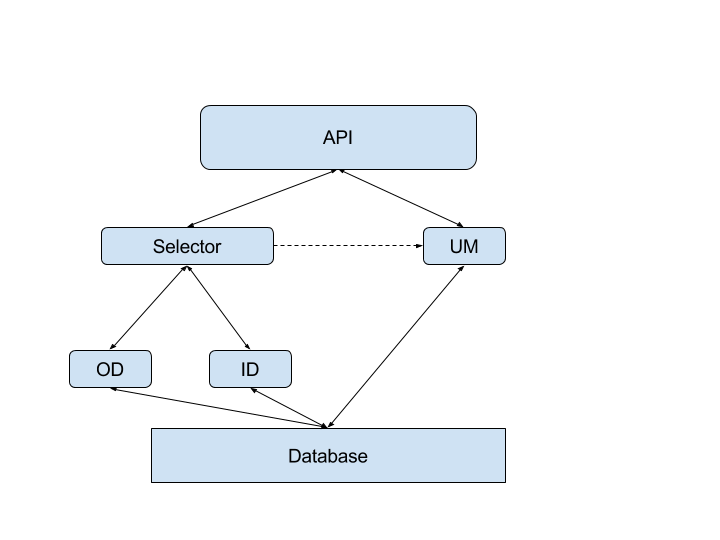
\includegraphics[width=\textwidth,trim={0 0 4cm 0},clip]{figures/InformalArchitecture.png}
		\caption{The \gls{astep} core architecture \cite{astepArchitectureImage}. }
		\label{fig:astepCore}
	\end{subfigure}
	~ %add desired spacing between images, e. g. ~, \quad, \qquad, \hfill etc. 
	%(or a blank line to force the subfigure onto a new line)
	\begin{subfigure}[b]{0.56\textwidth}
		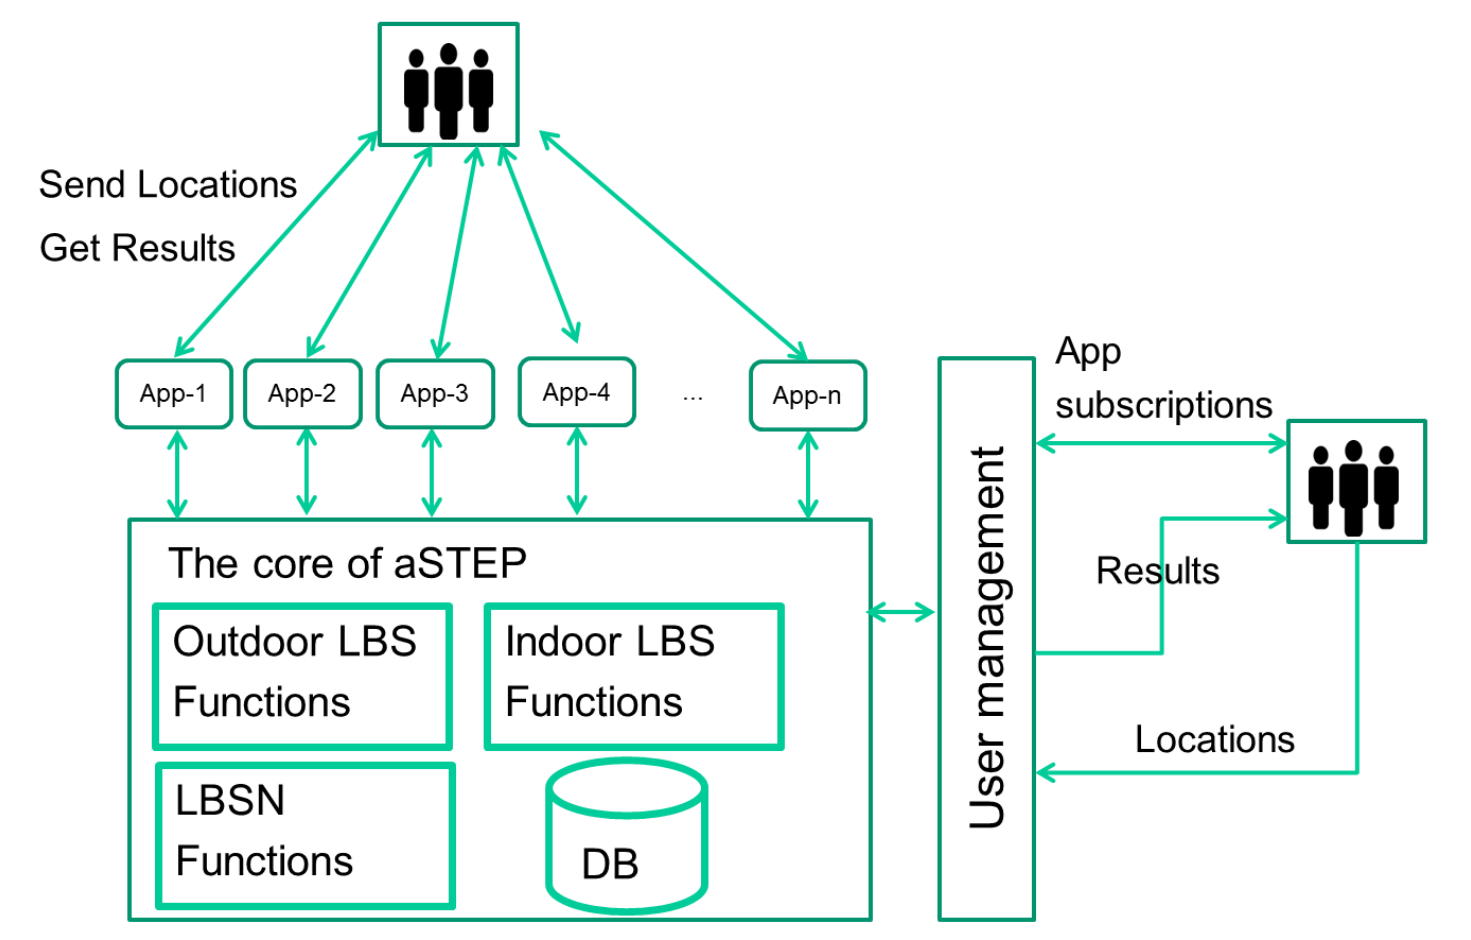
\includegraphics[width=\textwidth]{figures/astepGroups.png}
		\caption{The \gls{astep} group distribution according to the project guidelines.}
		\label{fig:astepGroups}
	\end{subfigure}
	\caption{\gls{astep} architectural design}
	\label{fig:astepArchitecture}
\end{figure}

Our project group is responsible for developing an app that utilizes the \gls{astep} core through the API, and contribute to the development of the interface of the core.
As the project focus is on commuting, the solution will depend upon outdoor location based services.
Any user registration, login or other user related tasks should be handled by the user management group.
According to our project focus and the component architecture, represented in Figure \ref{fig:astepCore}, we will mainly cooperate with the OD and user management groups.



% Sprint 1
\chapter{Sprint 1}
The first sprint is concerned with getting the semester project started, including both the \gls{astep} project as a whole and the \gls{rs} project.
Thus, the first sprint will be spent on organizing the collaboration with the other project groups and setting the direction for the project.
This means that the contributing parts of sprint 1 will be the initial analysis, requirement specification and overall design, with the documentation in this chapter in the same order.

\section{Analysis}
Ridesharing is an activity which has had phases of popularity in recent history according to \citet{doi:10.1080/01441647.2011.621557}.
They describe the current phase as the technology-enabled ridematching phase which started in 2004.
In this phase, the intergration of the internet, mobile phones, and social media has into ridesharing services, reduces the barrier to entry for new potential passengers and drivers.
\citet{doi:10.1080/01441647.2011.621557} also list incentives for ridesharing in the current phase, which are as follows 

\begin{itemize}
  \item ``Focus on reducing climate change, growing dependence on foreign oil, and traffic congestion
  \item Partnerships between ridematching software companies and regions and large employers
  \item Financial incentives for green trips through sponsors
  \item Social networking platforms that target youth
  \item Real-time ridesharing services'' \citep{doi:10.1080/01441647.2011.621557}.
\end{itemize}

This presents a broad overview of why ridesharing became popular again after 2004.
Because technologies play a vital role in the current phase a selection of popular commercial services will be examined a long with some scientific papers to get a comprehension of the state of the art in the field.
%The following section documents the analysis of both academic papers, as well as corporate and community products, to get a comprehension of the state of the art in the ridesharing field.
The main focus will be on real-time or dynamic ridesharing which \citet{amey2011real} defined as ``rideshare service relying heavily on mobile phone technologies''.

\subsection{Scientific Papers}
The problem of automating ridesharing through modern technology has already been studied by multiple scientists \todo{what?} with different approaches.
The following sections account for some of which we found the most interesting and relevant to the problem statement. 

\citet{doi:10.1080/01441647.2011.621557, amey2011real} sees technology as one of the most important factors in the present and future of dynamic ridesharing.

\citet{ShuoMa2013} developed an algorthm for taxi services which improved throghput of passengers by 25\% and reduced the distance a single taxi had to drive by 13\% when there where there were six requests for rides per taxi. %  picking up many passengers throughout a ride is developed and presented, seeking to increase the passenger throughput as well as lowering the distance traveled per passenger served.
Especially interesting in their paper is an approach which suggests a grid representation of a road network, this is to avoid shortest path calculations between points on a map, and instead approximate distance represented by cells in the grid.
The paper also uses	 the user's smartphone to collect location data and act as a user interface.

\citet{ghoseiri2011real} researched what might matter when matching driver and passengers.
They focused on preferences which influence whether you want to drive with a person, this can be everything from gender to pet friendliness.
They developed functions which assesses whether a passenger and driver match, based on location, preferences, passenger and/or driver detour as the most important factors \cite{ghoseiri2011real}.
This algorithm might be useful in this project solution.

Actual choices and influences regarding algorithm design for ridematching will be addressed in the design phase. 

\subsection{Commercial Solutions}
Corporate and community solutions are quite different from the academic field.
The main focus seems to be centered around taxi alternatives.
The two biggest international services in this field as of 2016 is Uber and Lyft\todo{source}.
There are also several services with some or all of their focus in Denmark, most notable is services like Haxi and Drivr\todo{source}.
These services work in a similar way: 

\begin{enumerate}
	\item A customer request a ride through an smartphone app or a web interface
	\item The backend of the service sends the request to one or more appropriate drivers
\end{enumerate}

Since the mentioned services are commercial and closed-source, actual information about the services design or architecture is not available.
Drivr has two interesting feature in comparison to their opponents, that is a web system for fleet management and business which provides administration and expense control of employee taxi travels.

Besides these taxi like services, there also exist services which focus on traditional ridesharing between private people where money is not earned.
Again, here exist both local and international services. 
These services give the opportunity to either offer a lift, request a ride and the possibility to connect drivers and passengers.
These services are usually free, but some of them charge a small fee when connecting people.
Some of the more notable are GoMore and iRideshare.\todo{source}

The smartphones have automatized much of the labor concerning organizing ridesharing and act as a central component in all the analyzed systems\todo{what?}.
However, we still see an opportunity to use the smartphone even further in a service that arranges rides between users, thus decreasing the required labor.
\section{Requirement Specification}\label{sec:req}
% Metatext
The requirements are divided into two main categories, functional and nonfunctional requirements, and are furthermore sorted in the MoSCoW \cite{moscow} structure.
The structure assists in solving the core purpose of the system first, as these are the highest prioritized requirements, and later adding additional functionality.


% Requirements
\subsection{Functional requirements}
The functional requirements are directly related to the tasks and operations of the developed application.

\textbf{Must-have requirements}\\
The 'Must have' requirements must be fulfilled for the solution to be acceptable.

\textit{Graphical user interface}\\
The application must have a graphical user interface (GUI) as users must be able to use the application themselves, and to structurally and aesthetically display user matches. 
The GUI must be intuitive as users may have different levels of experience with using mobile applications.

\textit{User accounts, including login and registration.}\\
Unique user accounts are required as it serves as an identifier for each user in the system. 
With user accounts, store personal information, and compare user based on the data. 
It will also provide functionality for displaying user to other users.

\textit{Communication with the \gls{astep} system.}\\
As the project is a part of the bigger system \gls{astep}, there must be a relation to the developed platform. 
The communication would be storing data in the \gls{astep} database and using user management also implemented on the platform.

\textit{User location tracking and storage.}\\
The application must track users as they move, to be able to determine the users travel routes.
The application should store the commuted routes and the data should be stored in the \gls{astep} database.

\textit{Automatically determine regular routes.}\\
The solution must automatically determine if a route is regular. 
Regular routes should be used for route comparison and match generating. 

\textit{Automatic user ridesharing suggestions.}\\
Automatic matching with other users routes must be provided to the the individual app users, and the matches must be computed.
When two regular routes are found similar, the users must receive an indication of the match in the app.
If the match computation shows to be a excessive process it is deemed to be done in the \gls{astep} core.


\textbf{Should-have requirements}\\
The requirements in this subsection are important, but are not regarded as critical for the functionality of the solution.

\textit{Give the user option to specify whether they have a car or not.}\\
Because some users might not have a car, they should be considered differently than the ones with, as the users without vehicle cannot give a ride to a potential match.

\textit{Enable users to blacklist other users.}\\
Users should be able to filter other users from the matches to prevent further possible bad experiences with either a driver or passenger.

\textit{Suggest rides with users who only drives a subset of the way from A to B.}\\
Giving users the option to match with people who do not have the same source and destination, will increase the number of suggested matches, as a user can join a part of the matches' route.


\textbf{Could-have requirements}\\
The 'Could have' requirements are the lowest realistically fulfillable requirements, and are implemented if the higher priority requirements are fulfilled.

\textit{Ride reservation or request from, to, time.}\\
This requirement enables the user to reserve rides with other users. 

\textbf{Would-have requirements}\\
The following requirements are only considered when all other requirements are satisfied but initially regarded as tasks to be solved in future projects.

\textit{Inform users of their environmental and economic savings due to their use of the solution.}\\
Provide users with detailed information on how much fuel the user has saved, how much money saved based on fuel prices, and how much CO2 that is not released into the environment. 

\subsection{Non-functional requirements}
The nonfunctional requirements for the solution are stated here.

\textbf{Must-have requirements}\\
These are the requirements the solution must fulfill to be acceptable.

\textit{Development cooperation with the other \gls{astep} project groups.}\\
The development must be done in cooperation with the other \gls{astep} groups.

\textit{User privacy}\\
The app must respect user privacy, especially in regards to a user location data and personal user data.
The solution should consider securing elements such as database storage, user management, and developers.

\textbf{Should-have requirements}\\
These requirements are important, but are not regarded as highly critical.

\textit{Aesthetics matching other \gls{astep} project applications}\\
The app should share design and guidelines as the other apps developed for \gls{astep}.

As the requirements for the solution now are documented the first design phase can be initiated. 
\section{Design}\label{sprint1design}
% Metatext
This section contains the overall app design, which is based on requirements with inspiration taken from the different commercial products and the papers read in the analysis.
The section will outline the main features of the design concerning system's structure, components, and user interface.

\subsection{System design}
To exploit the availability of sensors on the mobile phone and computational power of the server, the system is developed in two parts: the phone application and an extension of the route system in the \gls{astep} system which handles the analysis and comparison of routes.
The two parts will have their own delegated responsibilities, and will perform the necessary tasks, enabling the system to deliver the service.

% The app
\textbf{The \gls{rs} App}\\
The application, hereafter referenced as the app, is the program executed on a mobile device.
Its responsibilities include the gathering of location data and providing the user interface. 

% device limitations -> app abilities
The task of comparing routes is assumed to require much processing power, and also be able to access location data to get the aforementioned routes.
Performing the route comparisons in the app would require that each user have a copy of every other user's routes.
This is a serious privacy concern as this can enable other applications to leach on to the \gls{astep} system a gather data about when people are home and where they live, and is an aspect we would like to avoid.
As mentioned before, calculating the best route matches would most likely require a lot of processing power, which would drain the battery and produce heat.

Assuming that a central server can handle the analysis of the routes, the application is only required to supply the server with location data.
This is a much better solution as the impact on the battery is reduced, and private information can be contained within the \gls{astep} system.

A service running in the background of the app can handle the location data sampling and transfer to a server.
This service would be kept alive when the application is closed as its own thread, thus being able to record routes even when the app is not in focus on the device.
Because the main objective of the background service is to observe the current activity and transfer the route to \gls{astep}, we call it Observer.
The structure of the class can be seen in Figure \ref{fig:classDiagramSprint1Observer}.
The Observer's main goal is to observe what activity the user is currently performing and receive and push locations accordingly.
There are already implementations for this kind of service in Google Play Services for Android applications and these will be utilized.

\begin{figure}[h]
	\centering
	\input{figures/classDiagramSprint1Observer.tex}
	\caption{The small process which should run at all time to build the routes.}
	\label{fig:classDiagramSprint1Observer}
\end{figure}

The API does also have features for detecting which activity is currently being performed.
This can be used to stop and start the gathering of location data, depending on the given activity.

% The aSTEP core
\textbf{The \gls{astep} Component}\\
On the \gls{astep} server, the route is stored in a database and accessed by the RouteStabilityAnalyser.
This analyzer takes the route and compares it to other routes by the same user, to determine whether this route is a regular occurrence, and hence a stable route.

If the RouteStabilityAnalyser determines that the route is stable, the route should be marked with a tag indicating that the route is stable in the database together with values that indicate when this route is expected to occur next.
The server then uses the RouteSimilarityAnalyser to find matches for the new StableRoute.
The matches are stored and new matches are transmitted to the appropriate devices when possible to inform the users of new matches.

%\begin{figure}[h]
%	\centering
%	\input{figures/classDiagramSprint1Application.tex}
%	\caption{The class structure of the application.}
%	\label{fig:classDiagramSprint1Application}
%\end{figure}

This is the start of a project that will be further developed upon and expanded in the future, emphasizing the importance of reuse in the server, to reduce the number of specialized server resources.
By isolating parts that are specific to the rideshare app on the server, most of this system would be reusable.
An example of how this is achieved through object-oriented design, is the RouteAnalyser seen in Figure \ref{fig:classDiagramSprint1Server}.
The RouteAnalyzer filter routes according to its concrete implementation.
After the filtering, the RouteAnalyser compare the routes.
This enables other projects to develop their own filters and comparison functions for later projects.

\begin{figure}[h!]
	\centering
	\input{figures/classDiagramSprint1Server.tex}
	\caption{The structure of the system inside the server.}
	\label{fig:classDiagramSprint1Server}
\end{figure}

Because commuters were our target and commutes are most likely to occur on a weekly basis, a weekly stability was decided upon.
This means that the RouteStabilityAnalyser can be limited to analyze only two months of data, as the route can be stopped driven.

\subsection{User Interface Design}
% General Introduction to UI - what + why
The \gls{ui} provides interaction methods between the user and the app.
As the priority of this project is functionality with regards to data collection and route generation and comparison, the \gls{ui} will not be developed together with users, nor allocated excessive resources. 
The \gls{ui} is developed for practical purposes, such as testing, and to lay the basis for further development, but is still held to a usable standard which will be documented in the following sections. 

\subsubsection{Design language}
% Definition
The design language is the general look and appearance of a system.
This is the foundation for the user impressions and affects the user experience.
The design language is selected in collaboration with another aSTEP project group, SW604F16.

% Goals
The user interface is designed to achieve the following usability characteristics described by \citet{DIS2014}:
\begin{itemize}
	\item Learnability
	\item Utility
	\item Safety
	\item Effectiveness
\end{itemize}

% Material design
The \gls{ui} is designed to comply with the Google's Material design guidelines \cite{materialDesign}, being ``\textit{bold, graphic, intentional}''. 
Some of the Material design properties are stated in the following list, compiled of citations from the design guidelines \cite{materialProperties}:

\begin{enumerate}
	\item Material has varying x \& y dimensions (measured in dp) and a uniform thickness (1dp).
	\item Material casts shadows. Shadows result naturally from the relative elevation (z-position) between material elements.
	\item Content is displayed on material, in any shape and color. Content does not add thickness to material.
	\item Input events cannot pass through material.
	\item Material cannot pass through other material. For example, one sheet of material cannot pass through another sheet of material when changing elevation.
	\item Material grows and shrinks only along its plane.
	\item Material never bends or folds.
	\item Material can be spontaneously generated or destroyed anywhere in the environment.
\end{enumerate} 

% Paragraph regarding selection of material
Adhering the material design guidelines makes the app achieve a similar aesthetic and usage method as other apps in the Android eco-system. 
The design language aims to make the interface clean and simple, regarding colors and input methods.

\subsubsection{User interface}
% Actions in UI and design thereof
This section contains design drafts of the user interface style and functionality.
The design drafts in Figure \ref{fig:GUI-firstrun} reflect the necessary functions and the previously described design language. 

% Login and registering pages design
As the user needs a user profile in the \gls{astep} system to use the app, the users must be able to log in if they have a user profile, and create a new user profile if they are not already registered.

\begin{figure}[h!]
	 \centering
	 \begin{subfigure}[b]{0.3\textwidth}
	 	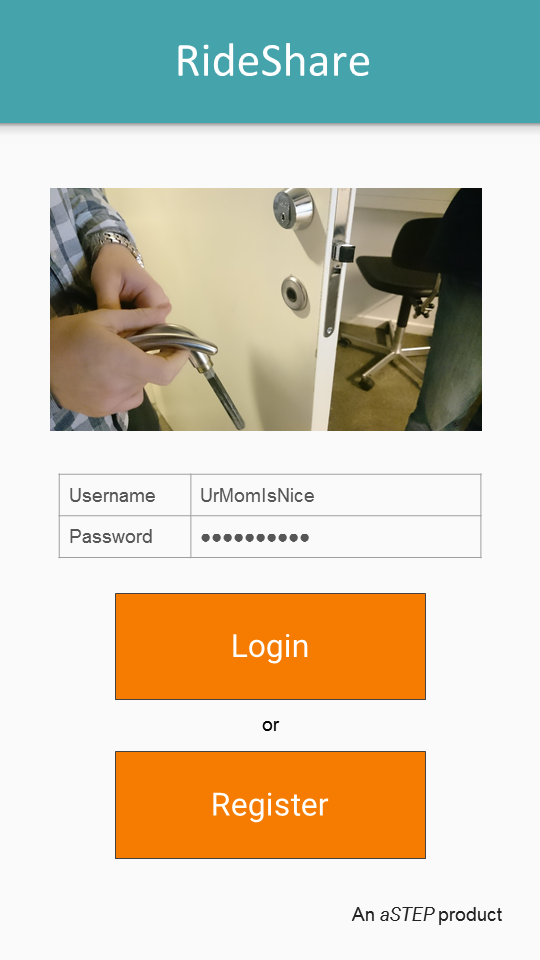
\includegraphics[width=\textwidth]{figures/GUI-front.png}
	 	\caption{Login page}
	 	\label{fig:GUI-front}
	 \end{subfigure}
	 ~ %add desired spacing between images, e. g. ~, \quad, \qquad, \hfill etc. 
	 %(or a blank line to force the subfigure onto a new line)
	 \begin{subfigure}[b]{0.3\textwidth}
	 	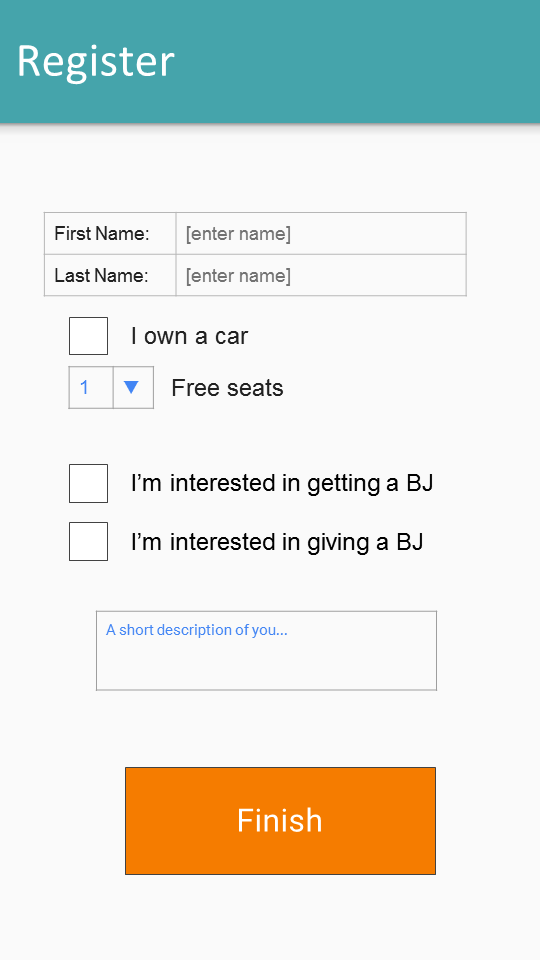
\includegraphics[width=\textwidth]{figures/GUI-register.png}
	 	\caption{Register page}
	 	\label{fig:GUI-register}
	 \end{subfigure}
	 ~ %add desired spacing between images, e. g. ~, \quad, \qquad, \hfill etc. 
	 %(or a blank line to force the subfigure onto a new line)
	 \begin{subfigure}[b]{0.3\textwidth}
		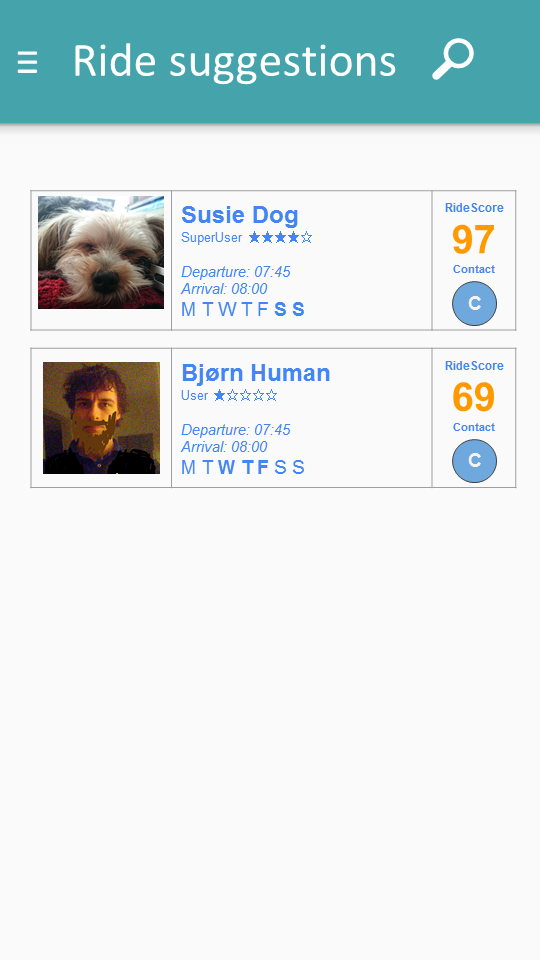
\includegraphics[width=\textwidth]{figures/GUI-main.png}
		\caption{Main page}
		\label{fig:GUI-main}
	\end{subfigure}
	 \caption{Draft of the views in the app.}\label{fig:GUI-firstrun}
\end{figure}

% In-app pages design
Several views are necessary to support the different parts of the app. 
The app needs views for login, registering, and presentation of matches as can be seen in the figures in Figure \ref{fig:GUI-firstrun}.

The application must be able to show matches in a separate view.
In this view, the user will be presented a list of other users which most likely are good matches. 
The users listed should be in a descending order, with the highest rated match at the top.
A short description of the users and match should be displayed, such as the user's full name, phone number, the match score, and what day(s) of the week the user drove the route and is expected to drive again.

This concludes the design of the app.
As earlier mentioned, the \gls{ui} is not the main focus of the project and will therefore not be further developed for other than functional purposes.

%\begin{figure}[h!]
%	\centering
%	\begin{subfigure}[b]{0.3\textwidth}
%		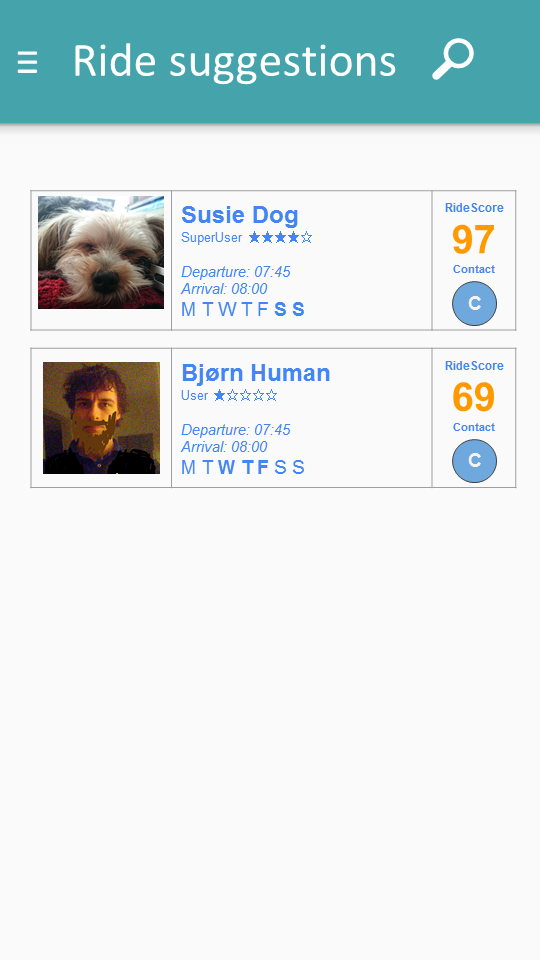
\includegraphics[width=\textwidth]{figures/GUI-main.png}
%		\caption{Main page}
%		\label{fig:GUI-main}
%	\end{subfigure}
%	~ %add desired spacing between images, e. g. ~, \quad, \qquad, \hfill etc. 
%	%(or a blank line to force the subfigure onto a new line)
%	\begin{subfigure}[b]{0.3\textwidth}
%		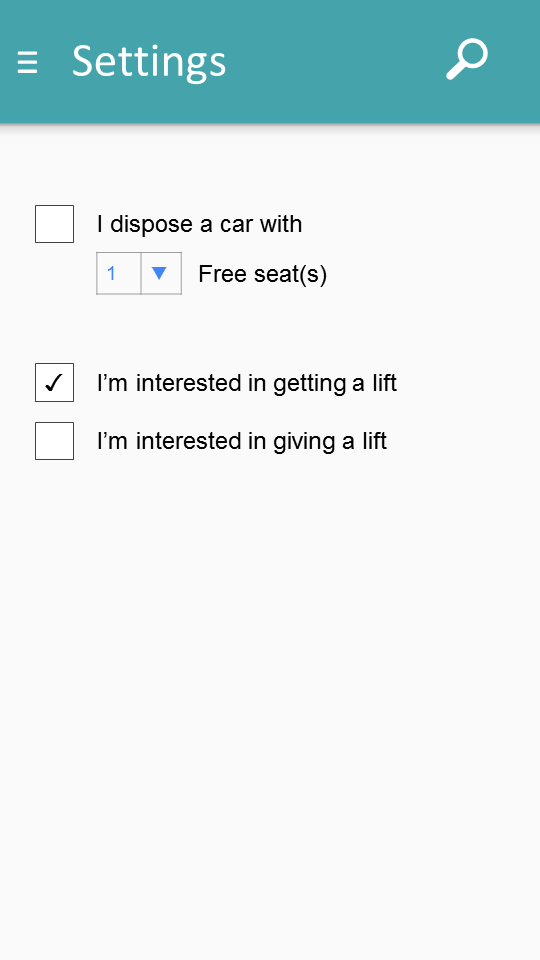
\includegraphics[width=\textwidth]{figures/GUI-settings.png}
%		\caption{Settings page}
%		\label{fig:GUI-settings}
%	\end{subfigure}
%	\caption{Draft of the views in the app.}\label{fig:GUI-in-app}
%\end{figure}
%\section{Implementation}
%\section{Test}

% Sprint 2
\chapter{Sprint 2}
\section{Analysis}
This section contains the analysis of app functionality, Android app development, \gls{rs} algorithms and communication with the aSTEP system.

%temporary title
\subsection{App functionality}
% meta shit
The app user interface is a low priority task during this project.
However, the app needs basic functionality, according to the requirements.

% Only vehicle
To concentrate the app focus and to ensure that users matched by routes can transport each other, the app is decided to only track a user when in a vehicle.
This excludes consideration of users only bicycling or walking as means of transportation.
The app could be expanded upon later, but at the current stage, only car commuters are targeted as app users.
% User management
To be able to separate different routes, and to assign them to their respective users, there has to be a user management system, so that each user has its own ID.
% Ride matches
The user should also be informed with relevant information of ride matches, so that the user can make a decision of sharing a ride or not.

% User settings
The user of the application should also be able to adjust their settings.
The settings are preferences regarding different properties of ride sharing.
The user should be able to decide if it wants to get a ride or give a ride or both.
There are also properties of the user itself, like a description and a picture, that other users can access to decide if they want to share a ride with the named user.

% other shit..

\subsection{Android Development Platform}
When developing Android applications one of the first choices to consider is which API levels to target \cite{usesSDK}.
The ``\textit{API Level is an integer value that uniquely identifies the framework API revision offered by a version of the Android platform.}'' according to Android Developers \cite{usesSDK}.
The distribution of the Android version levels are shown in \ref{fig:dashboard}.

``\textit{The manifest file presents essential information about your app to the Android system, information the system must have before it can run any of the app's code.}'', according to Android Developers \cite{androidManifest}.
The manifest requires to specify the API level for three definitions: minimum, target and maximum. 
The target and max versions requires few consideration to determine.
The ``targetSdkVersion'' reflects the version to which the app is developed and tested against, without enabling compatibility behaviors.
The ``maxSdkVersion'' reflects the highest API level that an app is designed to run.
Both of these are set to the highest API level available during the start of the development, which is API version 23.

The last API level which needs to be specified is the ``minSdkVersion''.
This entry specifies the lowest API level which an app supports.
A cause of this is that every device with an API level lower than the specified minSdkVersion will not be compatible with the app.
Supporting older API versions requires development efforts, typically implementing functionality though the Android Support Library \cite{androidSL}.
For this project we choose to target a higher API level for to simplify the development process.
At the time of writing, the platform version distribution sum of API levels greater than or equal to 21 (Android Lollipop) is 35,3\%.

\begin{figure}[h]
	\begin{center}
	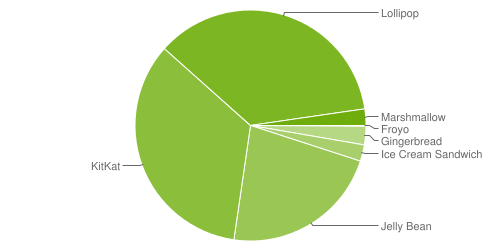
\includegraphics[width=0.78\textwidth]{figures/android-chart-march.png}
	\end{center}
	\caption{Android version distribution, March 2016 \cite{androidDashboard}}
	\label{fig:dashboard}
\end{figure}
The version distribution as of March 2016 can be seen on Figure \ref{fig:dashboard}
API version 21 is chosen as the minSdkVerison, the main reason for this choice is to minimize development time as API level 21 among other things added support for the material design style \cite{android5API}. Refraining from further backwards compatibility allows the focus of the project to be on the functionality of the app. 

\subsection{Periodic Background Tasks}\label{ssec:periodictasks}
When the app is installed on the device, the app needs to run a task to periodically collect location data.
\Citet{friesen2015android} writes how this can be done in the Android API by utilizing the AlarmManager and the JobSchedular.

\paragraph{AlarmManager}
The AlarmManager was created to handle alarms, and implemented as a general class that can call any task after one or multiple given time periods.
The alarm can be set to be reoccurring, thus gather a location with the given interval.

\paragraph{JobScheduler}
The JobScheduler was implemented in Android 5.0 (API 21) as an alternative to the AlarmManager.
The scheduler behaves in a similar way as the AlarmManager, but tries to batch the jobs together and execute them in bundles.
This means that the device can save power by avoiding going to sleep just to wake a short moment later, on the cost of time precision. 
While the AlarmManager has the option to occur at a exact time, the JobSchedular does not.

The JobScheduler is chosen as the basis for the background tasks, because the timing accuracy of the location data is not sensitive to minor deviations, in addition to the advantages of saving power features.

\subsection{Location tracking}\label{ssec:loctrack}
% metatext
In order to be able to locate a user and to construct routes, it is necessary to collect location data. 
Such collection of locations can be done by using already existing services, such as the Google Play Services.

% something
Location data in \gls{rs} is formatted in decimal coordinates in an array that represents a route from A to B.
There are several ways to collect location data. 
One of them is to manually develop a component to do so on the Android device, but the chosen solution is to utilize the already existing Google Play Services.

To use Google Play Services, a client library must be included in the app, and will communicate via inter-process communication to the Google Play Services. 

An advantage of the Google Play Services \cite{GapiOverview}, is that it will automatically receive silent updates regularly, to acquire new features and bug fixes to the used services, developed by Google, and this is illustrated in Figure \ref{fig:gapifigure}.
The Google Play Services are restricted, and are not supporting devices with Android versions lower than 2.3. 
This limits the backwards compatibility, but the app is already restricted to Android 5 and newer, and has no influence on the target audience.

\begin{figure}[h]
	\centering
	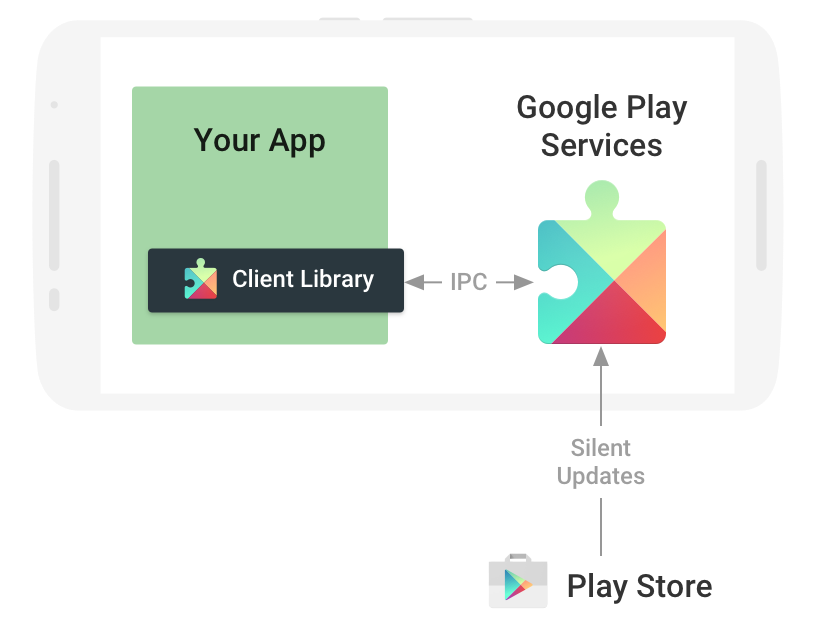
\includegraphics[width=0.7\textwidth]{figures/play-services-diagram.png}
	\caption{Google Play Services communication\cite{GapiFigure}}
	\label{fig:gapifigure}
\end{figure}

The Google Play Services will allow the application to collect location data, but it is not doing so solely by using the GPS in the device. 
The location service utilizes both network location and GPS to estimate a position as precise as possible \cite{GapiLocation}. 
To ensure the collected location data is relevant, locations are only collected when the user is traveling by vehicle.

The Google Play Services provides a service to determine the user's activity, called Activity recognition. 
Activity recognition is a service that utilizes several sensors on the device to determine what kind of activity the user is currently performing, therein driving, walking, etc.
The service will return a probability level from 1 to 100, where 100 is certain that a user is performing the activity.
The activity recognition will also prevent unnecessary data will be stored on the database. 

The practical design of the location tracking and activity recognition will be further explored in the following design section.
The \gls{astep} system is examined as an external tool, and its functionalities are explored.


% aSTEP system functionality analysis: communication with aSTEP
\subsection{Communication with \gls{astep}}\label{ssec:communicationwithastep}
To be able to utilize the \gls{astep} system, the communication protocol and its functions must be analyzed. 
The analysis is based on the current development and plan of the API and other functions.

% \gls{astep} organization - groups
The intended functions are established in collaboration with other project groups responsible for the \gls{astep} system side of the development. 
%We are mainly involved with the user management group and outdoor location based services groups.

% What does the \gls{astep} system look like?
The design of the \gls{astep} system is currently consisting of an API that apps and services can communicate with, and a backend with user management and location based services, which is stored in a database system.
However, the only relevant part for the \gls{rs} solution is the API, as the internal parts of the \gls{astep} core are administrated by other groups, and are not available through the API.

% What is stored in \gls{astep}
The \gls{astep} system will store information regarding location data, and basic user information. 
The data stored in the \gls{astep} system, relevant to this project solution, is:
\begin{itemize}
	\item Location data consisting of userID, routeID, GPS coordinates and timestamp.
	\item Username
	\item Password
\end{itemize}

The \gls{astep} user management system does not provide storage of data regarding contact information for \gls{astep} users.
The only information stored is a username and password to keep the \gls{astep} core as simple as possible.
Additional information that is required to make the app work as intended is each of the app groups own responsibility.
The \gls{astep} users are made to ensure the correct permissions are given to the correct user and so that the appropriate data is returned to each user.
An API call cannot be done without the user first being authenticated with a valid login.

% How to cummunicate with \gls{astep}
The communication with \gls{astep} is done through a REST API over HyperText Transfer Protocol, decided in agreement between the \gls{astep} project groups.
REST is an abbreviation of Representational State Transfer, and is a communication design often used in for HTTP-communication \cite{REST}.
Accordingly, the communication is performed by making queries to the \gls{astep} system. 
All communication must be done as a request from the device, to which the \gls{astep} server will respond.

% api functions
The currently available API functions at this stage of the development of \gls{astep} from user management and location services can be seen in Table \ref{tab:sprint2-api}.
The API is providing a POST-request under the name ``PostLocationDat'', as listed in \ref{tab:sprint2-api}, which is the current method to use when sending location data to the \gls{astep} system.
The call will accept location data as a coordinate consisting of longitude and latitude, a precision value, and a value representing time of day in milliseconds.

\begin{table}[!ht]
	\centering
	\begin{tabular}{ll}
		LBS & UM    \\
		\hline
		\begin{tabular}[t]{@{}l@{}}
			GetAllEntitiesInArea\\ GetAllEntitiesInTimePeriod\\ GetAllGroupMemebersLocationAndName\\ GetAllFriendsInArea\\ GetAllFriendsInRadius\\ GetAllGroupMembersInArea\\ GetAllGroupMembersInRadius\\ PostLocationData\end{tabular}
		&
		\begin{tabular}[t]{@{}l@{}}
			Create user\\ Get token\\ Update password\\ Edit privacy settings\\ Allow user2 to access user1's info\end{tabular}
	\end{tabular}
	\caption{Currently planned \gls{astep} API functions.}
	\label{tab:sprint2-api}
\end{table}


As both the \gls{astep} service and Android system have been analyzed it is possible to establish a set of requirements for the second sprint.

% Sprint 2 krav
\subsection{Requirements for the second sprint}
%meta
Sprint two is the first of the two middle sprints that have implementation as the primary focus. In this section, the main issues to be solved in the current iteration will be presented.

% algorithm
\textbf{Route Matching Algorithm}\\
In this sprint, the algorithm for comparing routes must be researched and developed. 
It should be developed to an extent so that it is constructed as pseudocode of the algorithm, to be handed over to another \gls{astep} group, and be implemented in the \gls{astep} system.

\textbf{User Data}\\
User information such as username, password, and login token, must be analyzed to figure out where this information should be stored, and how it should be handled regarding communication between the application and the aSTEP server. 

\textbf{RideShare app}\\
A base for the functionalities for the \gls{rs} application should be implemented. 
The implementation should include a working \todo{?} including of the Google Play Services and the application should be able to collect and store location data. 
The application should also have functionality to run as a background services, so that location data can be collected at all times.

\textbf{System Architecture and Communication}\\
Communication between the \gls{rs} application and \gls{astep} server should also be researched and an implementation of the communication should be initialized in this iteration, ensuring the next iteration will have a base for communication. 
It should be considered how to handle storing the collected location data and how much should be stored where, either on the device or on the \gls{astep} server.

\textbf{Mock Data}\\
If there is spare time during the sprint, it should be considered to acquire mock up location data related to mock up users. 
This data could be used in the third iteration to test if the algorithm works as intended.
\section{Design}

% metatext
This section contains documentation of the design of the \gls{rs} solution.
The parts to be designed in this sprint are the overall system design, reflecting the changes in the \gls{astep} system, and the algorithms to generate stable routes and route matches.

% System design
\subsection{System design}
% metatext
The rideshare solution is designed to consist of multiple parts.
This section contains descriptions of the different parts, and a definition of their responsibilities.

% Description of the solution
\begin{figure}[h]
	\centering
	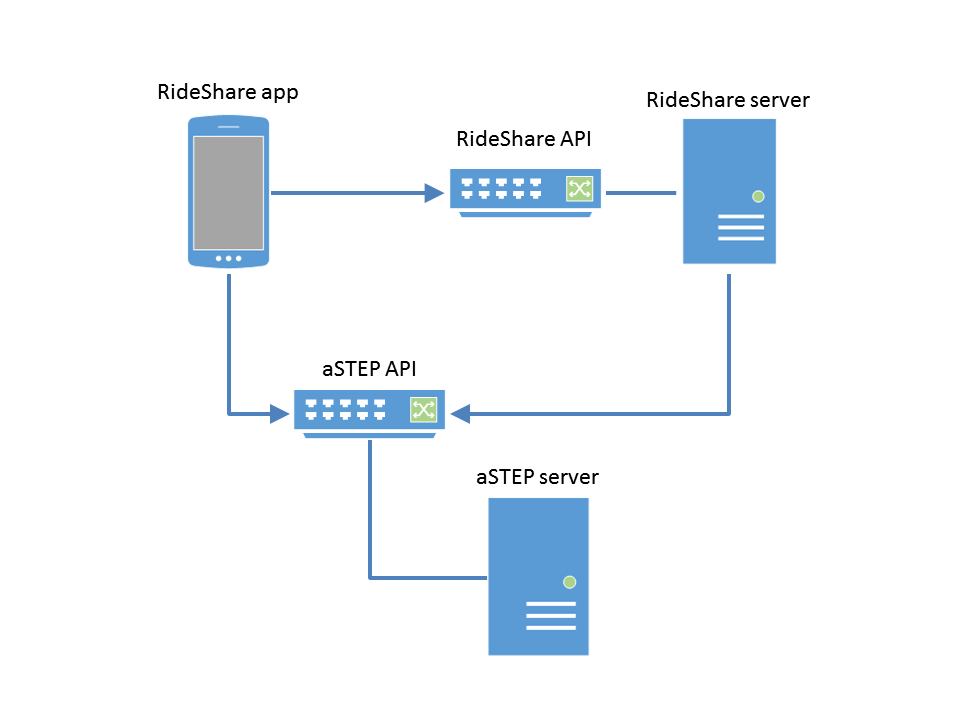
\includegraphics[width=\textwidth]{figures/SystemDesign.png}
	\caption{System design, including all major parts of the solution.}
	\label{fig:s2systemdesign}
\end{figure}

% Definition of APP responsibilities
The app...
Fetch route matches

% user management responsibilities
User interface for logging in, registering a new user, edit contact information.
Through RideShare server.

% location responsibilities
Provide aSTEP system with location data directly.



% Definition of RIDESHARE(TM) server responsibilities
RideShare server..

% user management responsibilities
Relay login request from app, save and relay the token.
Because the user management in aSTEP does not provide anything but username and password, the contact information and other data is stored on the RideShare server.


% location responsibilities
Fetch route matches for each user and store.



% Definition of aSTEP system responsibilities
aSTEP...

% user management responsibilities
Authenticate user by password.

% location responsibilities
Store locations, find stable routes, find route matches.


% Algorithm
\todo{This is a draft}

$\mathbb{L}$ is the set of all possible locations.

\begin{algorithm}
	\caption{The Time Analyser pseudocode}
	\begin{algorithmic}[1]
		\Require 
		\Statex $\delta\in \mathbb{R}_{>0}$ : the acceptable time difference
		\Statex $\gamma\in\mathbb{R}_{>0}$ : the translation from distance to time
		\Statex $dist : l_1,l_2 \in \mathbb{L} \rightarrow \mathbb{R}_{\geq 0}$ : the distance between $l_1$ and $l_2$
		\Statex $time : l_1,l_2 \in \mathbb{L} \rightarrow \mathbb{R}_{\geq 0}$ : the time difference between $l_1$ and $l_2$
		\Statex 
		\Function{TimeAnalyser}{$r, g$}
			\State $r_g \in r$ is the closest point to $g$
			\State $t_\delta\gets time(r_g, g) - 2\times dist(r,g)\times\gamma$;
			\State\Return $\frac{t_\delta}{\delta}$
		\EndFunction
	\end{algorithmic}
\end{algorithm}

Analysing the function Time Analyser we can see that on line 2 it should iterate over all locations in $r$ to make sure that $r_g$ is the closest possible point.
The complexity of this operation should be $\Theta(|r|)$ where $|r|$ is the number of locations in $r$.
Moving on to line 3 we have some basic arithmetic operations and the function call $time$.
A possible heuristic algorithm for time would be to find the distance between the two points and multiply it with the time it takes to travel one distance unit. 
This is an optimistic approach since it assumes that there is a path directly from $r_g$ to $g$.

In order to make this work for both stability and similarity

If this heuristic approach is used then the complexity of line 3 would be $\Theta(1)$.
Because line 4 is only using basic arithmetic operations then this line is also $\Theta(1)$ making the complexity of this function $\Theta(|r|)$.

 \begin{algorithm}
	\caption{The Distance Analyser pseudocode}
	\begin{algorithmic}[1]
		\Require 
		\Statex $\beta \in \mathbb{R}_{>0}$ : the acceptable detour length
		\Statex $dist : l_1,l_2 \in \mathbb{L} \rightarrow \mathbb{R}_{\geq 0}$ : the distance between $l_1$ and $l_2$
		\Statex 
		\Function{DistanceAnalyser}{$r, s, g$}
			\State $r_s \in r$ : the closest point to $s$
			\State $r_g \in r$ : the closest point to $g$
			\State $d_s\gets 2\times dist(r_s, s)$\Comment Pickup detour distance
			\State $d_g\gets 2\times dist(r_g, g)$\Comment Set off detour distance
			\State\Return $\frac{d_s + d_g}{\beta}$
		\EndFunction
	\end{algorithmic}
\end{algorithm}

The Distance Analyser uses a distance function.
This only need to be guiding so a heuristic function should be sufficient.
A possible implementation is to find the direct distance between the locations.
This would be a $\Theta(1)$ time function.
The function it self finds the closest points on route $r$ to the endpoints $g$ and $s$ in line 2 and 3.
This is done in $\Theta(|r|)$ time.
Line 4 and 5 uses the distance function which we earlier said was $\Theta(1)$, and line 6 uses basic arithmetic operations so the complexity of that is also $\Theta(1)$.
Making this functions complexity $\Theta(|r|)$.

\begin{algorithm}
	\caption{The Time Distance Analyser pseudocode}
	\begin{algorithmic}
		\Require 
		\Statex $d_\gamma\in \mathbb{R}_{>0}$ : the modifier for distance
		\Statex $t_\gamma\in\mathbb{R}_{>0}$ : the modifier for time
		\Statex 
		\Function{TimeDistanceAnalyser}{$r, s, g$}
			\State $d\gets$\Call{DistanceAnalyser}{$r, s, g$}
			\State $t\gets$\Call{TimeAnalyser}{$r, g$}
			
			\If{$d > 1 \vee t > 1$}
				\State $score\gets 1-\frac{d\times d_\gamma+t\times t_\gamma}{d_\gamma+t_\gamma}$
				\Comment $score \in [0, 1]$
				\State \Return $100\times score$
			\Else
				\State\Return 0
			\EndIf
		\EndFunction
	\end{algorithmic}
\end{algorithm}

The Time Distance Analyser uses the Time Analyser and Distance Analyser function which were defined as being $\Theta(|r|)$.
And then does a check and some arithmetic operations.
The limiting factor is the called functions so the complexity of this function must still be $\Theta(|r|)$.

\begin{algorithm}
	\caption{The Analyse Route pseudocode}
	\begin{algorithmic}
		\Require
		\Statex $scores(r, r') \rightarrow \mathbb{Z}$ : a matrix of scores between two routes
		\Statex
		\Procedure{AnalyseRoute}{$r, R$}
			\State $r_s\in r$ : the start point of route $r$
			\State $r_g\in r$ : the end point of route $r$
			\ForAll{$r'\in R$}
				\State $r'_s\in r'$ : the start point of route $r'$
				\State $r'_g\in r'$ : the end point of route $r'$
				\State $score(r', r)\gets$\Call{TimeDistanceAnalyser}{$r', r_s, r_g$}
				\State $score(r, r')\gets$\Call{TimeDistanceAnalyser}{$r, r'_s, r'_g$}
			\EndFor
		\EndProcedure
	\end{algorithmic}
\end{algorithm}

The final procedure takes in a route and a set of routes and calls the Time Distance Analyser two times for each route in $R$.
If we consider $\langle R \rangle$ to be the average length of all routes in $R$ and $|R|$ to be the number of routes in $R$.
Then the complexity would be $\Theta(|R|\times(\langle R\rangle + |r|))$.
$|r|$ could be represented within the average.
So the reduced complexity is $\Theta(|R|\times\langle R\rangle)$.
As the number of routes get greater the average route length gets harder to change between calculations and approaches therefore a constant value.
This means that as the set gets larger we approach this complexity $\Theta(|R|)$.

% Location gathering
\subsection{Location}
% metatext
In order to be able to locate a user and to construct routes, it is necessary to collect location data. 
The location data should only be collected under certain circumstances, such as when the user is driving in a vehicle. 
Such collection of location data can be done by using already existing services, such as the Google Play Service.

% something
Location data in RideShare is only useful if it is formatted in GPS coordinates, stored in a collection that represents a route from A to B.
There are several ways to collect location data. 
One of them is by developing a component to do so on the android device. 
Another way is to use already existing services, such as one of the Google Play Services.
%We have decided to use Google Play Services as they are well tested, and provide a reliable foundation.

To use Google Play Services, a client library much be included in the app, which will communicate via inter-process communication to the Google Play Services which is already existing on every android device. 
When the application is connected to the Google Play Services, it will automatically receive silent updates regularly, to acquire new features and bug fixes to the used services. 
This is illustrated in Figure \ref{fig:gapifigure}\cite{GapiOverview}.

\begin{figure}[h]
	\centering
	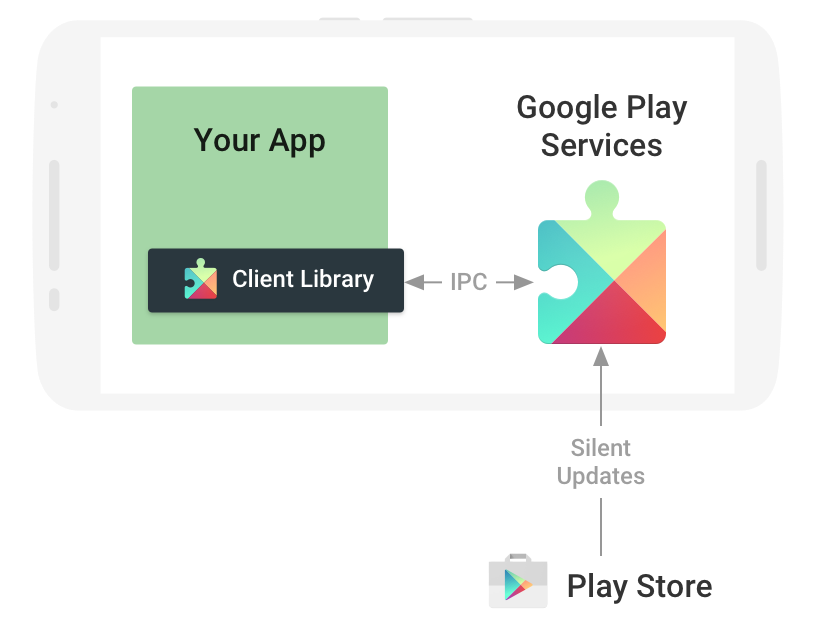
\includegraphics[width=0.7\textwidth]{figures/play-services-diagram.png}
	\caption{Google Play Services communication\cite{GapiFigure}}
	\label{fig:gapifigure}
\end{figure}

\todo{Skal måske flyttes}
The Google Play Services are restricted, and are not supporting devices with Android versions lower than 2.3. 
This limits the backwards compatibility, but the app is already restricted to Android 5 and newer, and has no influence on the target audience.
%This means that the application will not be backwards compatible as we have chosen only to focus on devices of Andorid version 2.3 and newer.

The Google Play Services will allow the application to collect location data, but it is not doing so solely using the GPS in the device. 
The location service utilizes both network location and GPS to estimate a position as precise as possible \cite{GapiLocation}. 
To ensure the collected location data is relevant, it is needed to store data only when the user is traveling by vehicle.
The Google Play Services provides a service to determine the user's activity, called Activity recognition. 

Activity recognition is a service that uses several sensors on the device to determine what kind of activity the user is currently performing, therein driving, walking, etc.
The service will return a probability level from 1 to 100, where 100 is certain that a user is performing the activity.
The activity recognition will be used to prevent unnecessary data will be stored on the database. 
%It may prevent some dirty data to be stored, that could be mistaken as routes from one location to another, which were not to be considered in this application in the first place.\todo{hard to understand} 
When a user is in a vehicle with a probability level above 75 \%\todo{placeholder}, data should be stored and used for computations.

The application must be running in the background while the device is turned on, for it to be able to differ between the users activity at all times and collect data. 
It is chosen only to collect location data from the location services every two minutes\todo{placeholder}, while in a vehicle, to reduce energy consumption. 
Every location collected during the driving activity must be appended to a list that represents an entire route when the driving activity ends.

When the activity change from vehicle to any other activity, the application will send the list of locations to the RideShare server, where it will take over the processing. 
\section{Implementation}
In this section we will document the initiating implementation of the \gls{rs} system, that has been designed until now. 
In this sprint the implementation of the location gathering as a background service will be documented. 

% Background service
\subsection{JobScheduler}

A JobScheduler works by getting a PendingIntent which contains information about what the user wants to happen and in what context.\todo{what is the intention/contents of this sentence?}
This is performed to ensure that any permission given is still available when the job is executed.\todo{source}

When a job\todo{what is a job?} is handed to the JobScheduler, information about the nature of the scheduling is also provided.
This includes requirements that needs to be fulfilled before the job can run, how often the job should be executed, and how precise the timing of the job should be.

The job itself can tell the scheduler how successful the job was, and if the job was unsuccessful and should be rescheduled.\todo{relevant?}

In the app, the job is implemented as an extension to the JobService class which provides the required interface for the JobScheduler called RideShareService.
The class reroutes the call by the JobScheduler to a Handler\todo{what is this?} class which handles the extension of the task in a separate thread.
The contents of this handler will be further explained later. \todo{Check that this line is correct.}


% Location gathering
\subsection{Location Gathering} \label{section:locationgathering}
% metatext
This section covers the implementation of the location gathering part of the background service.
To get the location of a device in a background service, the Google Play Services is utilized.
%The Google Play Services provides necessary location data, due to the integration on the platform.

% permissions
First, to retrieve location information, the \texttt{manifest.xml} file must be edited as to acquire permissions to the course and fine location.
When the manifest is set up correctly, the actual location retrieving can be performed.
This is done by adding the following lines to the manifest:
\begin{lstlisting}[language=XML]
<uses-permission android:name="android.permission.ACCESS_COARSE_LOCATION"/>
<uses-permission android:name="android.permission.ACCESS_FINE_LOCATION"/>
\end{lstlisting}

% gathering overview
The location is retrieved by utilizing the \texttt{GoogleApiClient}, then converted to an \gls{astep} location format.
This prepares the location data to be sent to the aSTEP system.


% googleApiClient
\textbf{Google API Client}\\
The \texttt{GoogleApiClient} is built and connected to when the \texttt{JobService} is created, hence performed in the \texttt{onCreate()} method, as the \texttt{JobService} thread only exists for the execution time of the contents.
The \texttt{GoogleApiClient} is disconnected in the method \texttt{onDestroy()} when the thread is terminated.

\iffalse
\begin{lstlisting}[caption={onCreate()},label={lst:oncreate},language=Java]
@Override
public void onCreate() {
	// Set the current Context to this
	context = this;
	// Builds the Google API Client to enable location
	buildGoogleApiClient();
	// Connects the Google API Client. It broadcasts to onConnect() when connected.
	connectApi();
}
\end{lstlisting}
\fi



% onConnected()
The \texttt{onConnected(Bundle bundle)} method is called when the Google API Client is ready.
When the client is ready, the \texttt{getCurrentGLocation()}, which can be seen in \ref{lst:onconnected}, is called, and the returned Android Location is stored in \texttt{currentGLocation}. 
The current Google location can then be stored in an aSTEP object, that later can be transmitted to the aSTEP system.

\begin{lstlisting}[caption={onConnected()},label={lst:onconnected},language=Java]
@Override
public void onConnected(Bundle bundle) {
	currentGLocation = getCurrentGLocation();

	// convert location to astep if available
	if (currentGLocation != null) {
		ASTEPLocation currentAstepLocation = convertToAstepLocation(currentGLocation);
	}
}
\end{lstlisting}


% getCurrentLocation()
\textbf{Get Location}\\
%To get the location of the device, the \texttt{getCurrentGLocation()} is called when the \texttt{onConnected(Bundle bundle)} receives the broadcast signal\todo{what?}.
The \texttt{getCurrentGLocation()} returns the last known location, according to the \texttt{googleApiClient}, in the Android Location format.
Before the location is gathered, because the target API is 23, the method needs to confirm the permissions required to acquire location data.
This is performed on line 6 and 7 seen on \ref{lst:getCurrentLocation}.
The device location is gathered through the \texttt{FusedLocationApi.getLastLocation()} method, using the \texttt{googleApiClient} as argument.

\begin{lstlisting}[caption={getCurrentLocation},label={lst:getCurrentLocation},language=Java]
private Location getCurrentGLocation(){
	Location tempGLocation = null;
	
	// Support Android M type permission handling
	try {
		if (ActivityCompat.checkSelfPermission(context, Manifest.permission.ACCESS_FINE_LOCATION) != PackageManager.PERMISSION_GRANTED &&
		ActivityCompat.checkSelfPermission(context, Manifest.permission.ACCESS_COARSE_LOCATION) != PackageManager.PERMISSION_GRANTED) {
			Log.d("BGS-LOC", "pass permission test");
			tempGLocation = LocationServices.FusedLocationApi.getLastLocation(googleApiClient);
		}
		
		// Get the current googleApiClient/LocationServices location
		tempGLocation = LocationServices.FusedLocationApi.getLastLocation(googleApiClient);
		
	}catch (Exception ex){
	}

return tempGLocation;
}
\end{lstlisting}

% aSTEP location
\textbf{Convert to aSTEP location}\\
The aSTEP location format contains the essential location information: latitude, longitude, accuracy, and a timestamp.
The \ref{lst:asteplocation} takes an Android location format data, creates an aSTEP location instance based on the argument location, and returns the aSTEP location.

\begin{lstlisting}[caption={ASTEPLocation()},label={lst:asteplocation},language=Java]
private ASTEPLocation convertToAstepLocation(Location gLocation) {
	Log.d("BGS-LOC", "convertToAstepLocation");
	ASTEPLocation aLocation = new ASTEPLocation(gLocation.getLatitude(),
	gLocation.getLongitude(),
	gLocation.getAccuracy(),
	gLocation.getTime());
	return aLocation;
}
\end{lstlisting}





\section{Test}



% Blah...

% Summary
\chapter{Summary}
\chapter{Summary}
This summary chapter contains the reflection, conclusion and further work.

\section{Reflection}
% metatext
This section contains our reflection of the different project aspects.
First, the project content and system design and implementation will be discussed.
Second, the work distribution and project process is described.

% project conten and system design/implementation
The system design was influenced by the \gls{astep} progression during the development.
Throughout the project time period, there were multiple changes in the \gls{astep} system, and they had different impact on our project.
Most significant was the change from \gls{astep} storing supplemental user information, such as e-mail address, to not providing other information than username and password.
The system design could have been better and there would be more time for implementation if the \gls{astep} system design had a static design from the beginning.

% project process and work distribution
The implementation was successful and dynamic, adjusting to changes made in the \gls{astep} project and our own tests performed in the iterations, in accordance with the iterative method.
All project members were somewhat included in every project project part.
Each member had a possibility to discuss the individual parts, despite being assigned to another part during that time period.
The tasks were evenly distributed on the group members, and more complex tasks were assigned two members, where necessary.

% project work load
We were ambitious with the extent of the project, therein objectives regarding custom user settings of having a car or not, despite the project leader Bin Yang proposed low ambition levels and just making a working basis.
Our ambition level is reflected in the requirement specification, 


\section{Conclusion}
% meta and contin. of introduction
The \gls{rs} solution, consisting of an Android application accommodated by an assisting server, utilizing the \gls{astep} system was developed in this project, and this section documents the conclusion of the project.


% conclusion on working process and cooperation
The \gls{astep} system was developed concurrently with the \gls{rs} solution, and both systems were dependent upon each other to be expedient.
The parallel development was influencing the development of the \gls{rs} solution, but also gave the possibility of establishing requirements for the \gls{astep} system.
The cooperation development process gave challenges as the other parts of the system were continuously altered, but a stable design was finally achieved and lead to a system that was functional.


% conclusion on the solution
The solution fulfills the established requirements regarding both functionality and cooperation with the other semester project groups, as stated in the test in Section \ref{sec:s4test}.
There is improvement potential for the solution, but the 'Must have' requirements are met, and the solution is acceptable in this regard.


% conclusion on the problem statement
The project has been focused on the problem statement, as defined in Section \ref{sec:probstat}:

{\addtolength{\leftskip}{10mm}\addtolength{\rightskip}{10mm}\noindent\hrulefill\it
	
	\noindent How can one design and develop an app that automatically suggests ride sharing companions, based on common locations in origin and destination, utilizing the \gls{astep} platform? 
	
	\noindent\hrulefill
	
}

The problem statement has been the initiating factor of the development process, and was assigned\todo{find better word} a set of requirements.
While the 'Must have' requirements are fulfilled, there are still remaining requirements regarding parts of the solution that are not completed.
However, the 'Must have' requirements were sufficiently covering the minimum level of functionality\todo{find synonym?}, and hence the problem statement is fulfilled and the solution is considered successfully accomplished.


% final conclusion
The semester project, solution, and the multi-group project lays the foundation for a potentially comprehensive location based service for both indoor and outdoor positioning.
Although the \gls{rs} app could benefit from a user interface redesign in terms of aesthetics, it solves the problem statement and can be applied in the real world.
\section{Future Work}
This section contains the features that were thought of during the project period, but were not implemented because of time constraints or disregarded to maintain a consistent focus for the project.

\subsection{Registration of users}
Because having connections between the users of the app and the \gls{rs}'s \gls{astep} user does not make any difference in the current version of \gls{astep}, the edges described in Section ?? \todo{} was not implemented.
This should be done during user registration with a few API calls.
It might be possible to also include a way to intergrate facebook as a alternative login method.

Another feature that is going to be important in the future is to allow users to use the same \gls{astep} user for multiple applications.
This can be done by introducing a two step registration, with the first step being logging in to \gls{astep} or creating a new \gls{astep} user.
And the second step being creating a new \gls{rs} user.
How this is achived is up to the group implementing it, but it could be done though an altered user interface.

\subsection{User interface}
And when talking about user interface.
It is stated multiple times that the focus of this project was never the interface, and it could therefor use an overhaul.
This overhaul would include a more consistent design between views and possibly a number of functionality that makes the app more enjoyable to use.

This could be profile pictures for matches, making the user more confident in that the person they are driving with is the same they matched with.
Another feature would be to display additional information when a user tapped on a match, a new activity would start which shows formation about the match.
This information could include other people that often travels with the user and details about the others route which were matched with.
One way to display details about the route that were matched witch would be to plot it into some sort of Google Maps intergration.

The app also does not take into account the users which are not driving.
This feature would require a rework of the internal route system in the \gls{astep} system.
Another thing that could be improved is the error messages displayed to the user, which currently is mostly non-informative or non-existent.

\subsection{Server}
To make the changes to the user interface a rework of some of the parts in the server would also need to be reworked.
Currently, there is no way to store profile pictures, and only meta data about routes are stored.
This means that there is currently no way to implement profile pictures, and there is not enough information in the meta data to plot the routes on a map.



%Register users på den rigtige måde med edges
%App
%	UI
%		Proper error handling/messages to user
%		App instruction pop-ups on first start
%	map view af ruter der er matched med
%	Vis profilbilleder
%Flyt overførslen af router over til body istedet for URL
%RSS
%	Gem profilbilleder
%	Push route matches
%Astep aka Algorithm
%	Display matches both ways?
%	Optimizations (d-trees?)
%	Grid/cell structure
%	Map integration (actual road distances and speed limits)
% Tag højde for folk der kører og ikke kører


% Bibliography
\printbibliography[heading=bibintoc]
\label{bib:mybiblio}

% Appendix
\appendix
\chapter{Database Implementation}
\label{appendix:database}
\begin{lstlisting}[
           language=SQL,
           showspaces=false,
           basicstyle=\ttfamily,
           numbers=left,
           numberstyle=\tiny,
           commentstyle=\color{gray}
        ]
CREATE DATABASE ramsydata;
CREATE TABLE userdetails(
	username VARCHAR(50) PRIMARY KEY,
	fullname VARCHAR(255),
	phonenumber VARCHAR(30),
	email VARCHAR(255)
);
?
CREATE TABLE matches(
	user1 VARCHAR(50) REFERENCES userdetails(username),
	user2 VARCHAR(50) REFERENCES userdetails(username),
	matchfound DOUBLE PRECISION,
	lastUpdate TIMESTAMP,
	score INT,
	PRIMARY KEY(user1, user2, matchfound)
);
\end{lstlisting}
\chapter{Appendix A name}\label{ch:appAlabel}
Here is the first appendix
\chapter{Sprint 4 \gls{rs} database test data}
\label{app:datadump}
\begin{lstlisting}[
           language=SQL,
           showspaces=false,
           basicstyle=\ttfamily,
           numbers=left,
           numberstyle=\tiny,
           commentstyle=\color{gray}
        ]
SET statement_timeout = 0;
SET lock_timeout = 0;
SET client_encoding = `UTF8';
SET standard_conforming_strings = on;
SET check_function_bodies = false;
SET client_min_messages = warning;
SET row_security = off;
-- Name: plpgsql; Type: EXTENSION; Schema: -; Owner: 
CREATE EXTENSION IF NOT EXISTS plpgsql WITH SCHEMA pg_catalog;
-- Name: EXTENSION plpgsql; Type: COMMENT; Schema: -; Owner: 
COMMENT ON EXTENSION plpgsql IS 'PL/pgSQL procedural language';

SET search_path = public, pg_catalog;
SET default_tablespace = '';
SET default_with_oids = false;
-- Name: matches; Type: TABLE; Schema: public; Owner: postgres
CREATE TABLE matches (
    user1 character varying(50) NOT NULL,
    user2 character varying(50) NOT NULL,
    matchfound double precision NOT NULL,
    lastupdate timestamp without time zone,
    score integer
);
ALTER TABLE matches OWNER TO postgres;
-- Name: userdetails; Type: TABLE; Schema: public; Owner: postgres
CREATE TABLE userdetails (
    username character varying(50) NOT NULL,
    phonenumber character varying(30),
    email character varying(255),
    fullname character varying(255)
);
ALTER TABLE userdetails OWNER TO postgres;
-- Data for Name: matches; Type: TABLE DATA; Schema: public; Owner: postgres
COPY matches (user1, user2, matchfound, lastupdate, score) FROM stdin;
niels	alex	1463383750000	2016-05-16 07:29:37.902	20
alex	carsten	1463383750000	2016-05-16 07:29:37.984	50
svend	carsten	1463383750000	2016-05-16 07:29:37.986	70
svend	alex	1463383750000	2016-05-16 07:29:37.987	90
test	alex	0	2016-05-16 15:33:19.818857	23
test	alex	1	2016-05-16 15:33:19.818857	47
test	carsten	1	2016-05-16 15:33:19.818857	3
test	carsten	21	2016-05-16 15:33:19.818857	87
\.
-- Data for Name: userdetails; Type: TABLE DATA; Schema: public; Owner: postgres
COPY userdetails (username, phonenumber, email, fullname) FROM stdin;
test	+4511223344	\N	Susie Hund
alex	+4512345678	\N	Alex
carsten	+4512345678	\N	Carsten
svend	+4512345678	\N	Svend
niels	+4512345678	\N	\N
wiingreen	+4542267385	\N	Claus Worm Wiingreen
\.
-- Name: matches_pkey; Type: CONSTRAINT; Schema: public; Owner: postgres
ALTER TABLE ONLY matches
    ADD CONSTRAINT matches_pkey PRIMARY KEY (user1, user2, matchfound);
-- Name: userdetails_pkey; Type: CONSTRAINT; Schema: public; Owner: postgres
ALTER TABLE ONLY userdetails
    ADD CONSTRAINT userdetails_pkey PRIMARY KEY (username);
-- Name: matches_user1_fkey; Type: FK CONSTRAINT; Schema: public; Owner: postgres
ALTER TABLE ONLY matches
    ADD CONSTRAINT matches_user1_fkey FOREIGN KEY (user1) REFERENCES userdetails(username);
-- Name: matches_user2_fkey; Type: FK CONSTRAINT; Schema: public; Owner: postgres
ALTER TABLE ONLY matches
    ADD CONSTRAINT matches_user2_fkey FOREIGN KEY (user2) REFERENCES userdetails(username);
-- Name: public; Type: ACL; Schema: -; Owner: postgres
REVOKE ALL ON SCHEMA public FROM PUBLIC;
REVOKE ALL ON SCHEMA public FROM postgres;
GRANT ALL ON SCHEMA public TO postgres;
GRANT ALL ON SCHEMA public TO PUBLIC;
\end{lstlisting}
\end{document}